\documentclass{report}
\usepackage{ressources/packages/miseEnPage}
\usepackage{ressources/vocabulaire/vocabulaire}

\pdfminorversion=4
\usepackage[francais]{babel}
\usepackage[utf8]{inputenc}
\usepackage[T1]{fontenc}
\usepackage{graphicx}
\usepackage{fancyhdr}
\usepackage{pdfpages}
\usepackage{float}
\usepackage{diagbox}
\usepackage[urlcolor=blue, linkcolor=black,linktoc=all, colorlinks=true]{hyperref}
\usepackage[left=2.5cm, right=2.5cm, top=2.5cm, bottom=2.5cm, headheight=15pt]{geometry}
\usepackage[final]{pdfpages}
\usepackage{helvet}
\usepackage{lscape}
\usepackage{wasysym}
\usepackage[multidot]{grffile}

\renewcommand{\familydefault}{\sfdefault}

\makeatletter
\def\@makechapterhead#1{% chapter
  \vspace*{5\p@}
  {
    \parindent \z@ \raggedright \normalfont
    \ifnum \c@secnumdepth >\m@ne
    \huge\bfseries \@chapapp\space \thechapter
    \par\nobreak
    \vskip 5\p@
    \fi
    \interlinepenalty\@M
    \Huge \bfseries #1\par\nobreak
    \vskip 10\p@
    \thispagestyle{fancy}% Permet d'ajouter l'entête de pied de page
  }
}

\def\@schapter#1{
  \if@twocolumn
  \@topnewpage[\@makeschapterhead{#1}]
  \else
  \@makeschapterhead{#1}
  \@afterheading
  \fi
}

\def\@makeschapterhead#1{% chapter*
  \vspace*{5\p@}
  {
    \parindent \z@ \raggedright
    \normalfont
    \interlinepenalty\@M
    \Huge \bfseries  #1\par\nobreak
    \vskip 10\p@
    \thispagestyle{fancy} % Permet d'ajouter l'entête de pied de page
  }
}
\makeatother


\usepackage[utf8]{inputenc}
\usepackage[T1]{fontenc}
\usepackage[francais]{babel}
\usepackage{graphicx}
\usepackage{listings}
\usepackage{color}
\usepackage{amsthm}
\usepackage{amsmath}
\usepackage{amssymb}
\usepackage{verbatim}

\definecolor{mygreen}{rgb}{0,0.6,0}
\definecolor{mygray}{rgb}{0.5,0.5,0.5}
\definecolor{mymauve}{rgb}{0.58,0,0.82}

\begin{document}
\lstset{ %
  backgroundcolor=\color{white},   % choose the background color; you must add \usepackage{color} or \usepackage{xcolor}
  basicstyle=\footnotesize,        % the size of the fonts that are used for the code
  breakatwhitespace=false,         % sets if automatic breaks should only happen at whitespace
  breaklines=true,                 % sets automatic line breaking
  captionpos=b,                    % sets the caption-position to bottom
  commentstyle=\color{mygreen},    % comment style
  deletekeywords={...},            % if you want to delete keywords from the given language
  escapeinside={\%*}{*)},          % if you want to add LaTeX within your code
  extendedchars=true,              % lets you use non-ASCII characters; for 8-bits encodings only, does not work with UTF-8
  frame=single,                    % adds a frame around the code
  keepspaces=true,                 % keeps spaces in text, useful for keeping indentation of code (possibly needs columns=flexible)
  keywordstyle=\color{blue},       % keyword style
  language=SQL,                 % the language of the code
  morekeywords={*,...},            % if you want to add more keywords to the set
  numbers=left,                    % where to put the line-numbers; possible values are (none, left, right)
  numbersep=5pt,                   % how far the line-numbers are from the code
  numberstyle=\tiny\color{mygray}, % the style that is used for the line-numbers
  rulecolor=\color{black},         % if not set, the frame-color may be changed on line-breaks within not-black text (e.g. comments (green here))
  showspaces=false,                % show spaces everywhere adding particular underscores; it overrides 'showstringspaces'
  showstringspaces=false,          % underline spaces within strings only
  showtabs=false,                  % show tabs within strings adding particular underscores
  stepnumber=2,                    % the step between two line-numbers. If it's 1, each line will be numbered
  stringstyle=\color{mymauve},     % string literal style
  tabsize=2,                       % sets default tabsize to 2 spaces
  title=\lstname                   % show the filename of files included with \lstinputlisting; also try caption instead of title
} 

\couverture{}
\pagestyle{pageNormale}

\setcounter{page}{1}
\tableofcontents{}

\chapter{Definitions}

\section{General definitions}
    \subsection{Graph}
        A graph is a pair (V, E) with a incidence relation $\sim$ such that:
        \begin{enumerate}
            \item V, E are finite sets
            \item $\forall e \in E, \exists !$ 1 or 2 element(s) $v \in V | e \sim v$
        \end{enumerate}
    \subsection{Vertex}
        A vertex of G is an element of V=V(G)
    \subsection{Edge}
        A edge of G is an element of E=E(G)
    \subsection{End of an edge}
        \[\begin{array}{r c l}
            v \sim e & \iff & v \text{ is incident with }e \\
            & \iff & v\text{ is an end of }e
        \end{array}\]
    \subsection{Parallelism}
        If 2 edges e and f have the same set of ends, e and f are parallels
    \subsection{Simple graph}
        A simple graph is a graph without any parallels edges or loop
    \subsection{Adjacent}
        Two vertex $v$ and $w$ are adjacent if $\exists$ one edge whose set of its ends is equal to ${v, w}$\\
        \begin{figure}[h]
            \centering
            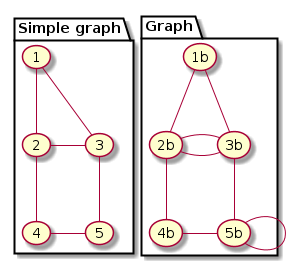
\includegraphics[scale=0.5]{ressources/images/GraphSimpleGraph.png}
            \caption{Simple graph $\Leftrightarrow$ Graph}
            \label{Simple graph & Graph}
        \end{figure}

\section{Type of graph}
    \subsection{Isomorphism}
        2 graphs G and H are isomorphic is $\exists \phi : V(G) \cup E(G) \rightarrow V(H) \cup E(H)$ bijective, such that:
        \begin{enumerate}
            \item $\phi(v)\in V(H)$ with $v\in V(G)$
            \item $\phi(e)\in E(H)$ with $e\in E(G)$
            \item $e\underset{G}{\sim}v \iff \phi(e)\underset{H}{\sim}\phi(v)$
        \end{enumerate}
    \subsection{Complete graph ($K_n$)}
        A complete graph is a simple graph with n vertex (for $K_n$) suc that every pair of distinct vertex are adjacent\\
        \begin{figure}[h]
            \centering
            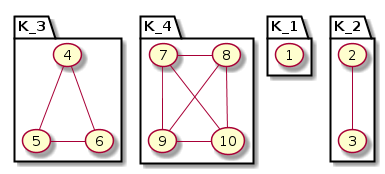
\includegraphics[scale=0.5]{ressources/images/CompleteGraphs.png}
            \caption{Every complete graph from $K_0$ to $K_4$}
            \label{Complete graph}
        \end{figure}
    \subsection{Subgraph}
        A graph H is a subgraph of G if:
        \begin{enumerate}
            \item $V(H)\subseteq V(G)$
            \item $E(H)\subseteq E(G)$
            \item  $\forall e \in E(H)$, the set of ends of $e$ in $H$ is equals to the set of ends in G
        \end{enumerate}
    \subsection{Spanning subgraph}
        A subgraph $H$ of $G$ is spanning if $V(H)=V(G)$
    \subsection{subgraph}
        A subgraph $H$ of $G$ is spanning if $V(H)=V(G)$

\section{Operations}
    \subsection{Deletetion}%TODO
    \subsection{Contraction}
        $G/e$ is the subgraph obtained from $G$ bydeleting $e$ and identitfying the 2 ends of $e$\\
        $|E(G)|=|E(G/e)|-1$\\
        $|V(G)|=|V(G/e)|-1$ (if e is not a loop)\\
        \begin{figure}[h]%TODO
            \centering
            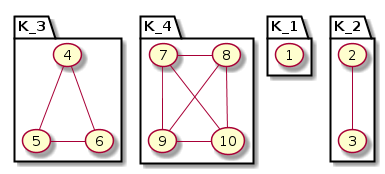
\includegraphics[scale=0.5]{ressources/images/CompleteGraphs.png}
            \caption{Every complete graph from $K_0$ to $K_4$}
            \label{Complete graph}
        \end{figure}
    \subsection{Minor}
        $H$ is a \textbf{minor} of $G$ if $H$ can be obtained from $G$ by deleting edges/vertices and contracting edges
    \subsection{Subdivision}
    $H$ is a \textbf{subdivision} of $G$ if $H$ can be obtain by subdivising somme edges of $G$\\
    $H$ is a \textbf{subdivision} of $G$ if $H$ can be obtained from $G$ by replacing each edge with a path of length $\geq 1$
        \begin{figure}[h]
            \centering
            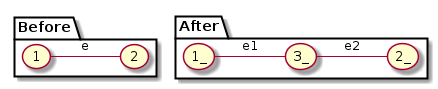
\includegraphics[scale=0.5]{ressources/images/SubDivision.png}
            \caption{Every complete graph from $K_0$ to $K_4$}
            \label{Complete graph}
        \end{figure}
    \subsection{Topological minor}
        $H$ is a \textbf{topological minor} of $G$ if a subdivision of $H$ is a subgraph of $G$\\
            \[\begin{array}{ccccc}
                \text{Subgraph} & \Rightarrow & \text{topological minor} & \Rightarrow & \text{minor}\\
                & \not\Leftarrow & & \not\Leftarrow & 
            \end{array}\]


\chapter{Connectedness}

\section{Definitions}
    \subsection{Walk}
        For 2 vertices $v$ and $w$, a \textbf{walk} from $v$ to $w$ is an alternating sequence $v_0 e_1 v_a e_1 \cdots e_n v_n$ of vertices $v_0, \cdots, v_n$ and edges $e_1, \cdots, e_n$. such  that the sets of ends of $e_i$ is {$v_{i-1} , v_i$} and $v_0 =v, v_n=w, n \geq 0$
    \subsection{Trail}
        A \textbf{trail} is a walk without using the same edge twice
    \subsection{Path}
        A \textbf{path} is a walk not using any vertex twice
    \subsection{Closed trail}
        A walk from $v$ to $w$ is \textbf{closed} if $v=w$
        A \textbf{circuit} is also a closed trail
    \subsection{Cycle}
        A \textbf{cycle} is a circuit $v_0 e_1 v_a e_1 \cdots e_n v_n$ such that $v_0, v_1, \cdots, v_{n-1}$ are distinct\\
        $Circuit\Rightarrow cycle$\\
        $Circuit\not\Leftarrow cycle$
\section{Theorems}
    \subsection{Lemma}
        \subsubsection{Definition}
             If $G$ has a walk from $x$ to $y$, then $G$ has a path from $x$ to $y$
        \subsubsection{Proof}
            \textbf{Induction on n}\\
            Let's call n the length of the walk $W$ from $x$ to $y$

            \begin{enumerate}
                \item If $n = 0$ : trival
                \item If $n \neq 0$ :
                    We may assume $W$ is not a path (Else, trivial)\\
                    $W$ has a vertex $z$ that is visited more that once.\\
                    $\begin{array}{c}
                        x=v_0 e_1 v_1 e_2 \cdots z \cdots z \cdots e_n y \\
                        \Downarrow\\
                        W'=v_0 e_1 v_1 e_2 \cdots z \cdots e_n y
                    \end{array}$\\
                    $W'$ is a walk from $x$ to $y$ whose length is $<$ $n$\\
                    By the induction hypothesis, $G$ has a path from $x$ to $y$\\
                    $G$ is connected $\Leftrightarrow \forall x, y \in V(G), G$ has a path from $x$ to $y$
            \end{enumerate}
            

    \subsection{$\sim$ relation}
        \subsubsection{Definition}
            $\forall x,y \in V(G), x \sim y \Leftrightarrow G$ has a path from $x$ to $y$
        \subsubsection{Equivalent ?}
        \[ \left \{
            \begin{array}{l}
                \textbf{symmetric}: x\sim y \Rightarrow  y\sim x\\
                \textbf{reflexive}: x\sim x\\
                \textbf{transitive}: x\sim y, y\sim z \Rightarrow x\sim z
            \end{array}
        \right .\]
    \subsection{Connected component graph}
        A \textbf{connected component} of a graph $G$ is a subgraph induced on an equivalence class of $(V(G), \sim)$\\
        i.e. : a component is a maximal connected subgraph
        \begin{itemize}
            \item If $C, D$ are component, then $C=D$ or $V(C) \cap V(D) = \emptyset$
            \item $G$ is disconnected $\Leftrightarrow V(G)$ can be partitionned into $A$ and $B$ (i.e. $A\cup B =V(G), A \cap B = \emptyset$) such that $A, B \neq \emptyset$ such that $G$ has no edge having one end in $A$ and another on $B$
        \end{itemize}
    \subsection{Forest and tree}
        ``Minimally connected'' graph $\sim$ tree
        \subsubsection{Tree}
            A \textbf{tree} is a connected graph with no cycle
            \begin{figure}[h]
                \centering
                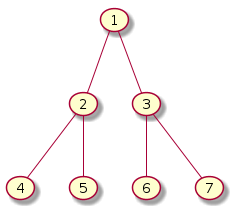
\includegraphics[scale=0.5]{ressources/images/Tree.png}
                \caption{A tree}
                \label{Tree}
            \end{figure}
            \subsubsection{Forest}
            A \textbf{forest} is a graph with no cycle\\
            \begin{figure}[h]
                \centering
                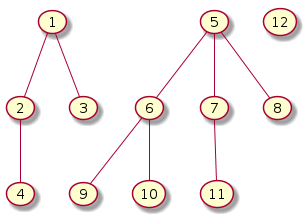
\includegraphics[scale=0.5]{ressources/images/Forest.png}
                \caption{A forest}
                \label{Forest}
            \end{figure}
        \subsubsection{Equivalence on trees}
            The following are equivalent: \\
            \begin{enumerate}
                \item $T$ is a tree
                \item $T$ is loopless and for $v, w \in V(T)$, $T$ has a UNIQUE path from $v$ to $w$
                \item $T$ is connected and $T$\\$e$ is disconnected from all $e\in E(T)$
                \item $T$ has no cycle and $T + xy$ (adding a new edge $xy$ to $T$) has a cycle for any $x, y \in V(G)$
            \end{enumerate}
        \subsubsection{Lemma}
            If $T$ is a tree with at least 1 vertex, then $|E(T)|=|V(T)|-1$
        \subsubsection{Proof}
            Induction on $|E(T)|$\\
            If $E(T)=\emptyset, \Rightarrow|V(T)|=1\Rightarrow 1-1=0$\\
            Now let $e\in E(T)$\\
            $T\backslash e$ has exactly 2 components $T_1, T_2$\\
            $|E(T_1)|=|V(T_1)|-1$\\
            $|E(T_2)|=|V(T_2)|-1$\\
            \begin{figure}[h]
                \centering
                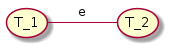
\includegraphics[scale=0.5]{ressources/images/BipartiteGraph2.png}
                \caption{A bipartite graph (With its 2 parts)}
                \label{Bipartite graph}
            \end{figure}
        \subsubsection{Corrolary}
            If $T$ is a tree with at least 2 vertices, then $T$ has a leaf
    \subsection{Bipartite graphs}
        $G$ is a \textbf{bipartite} graph if $G$ has a \textbf{bipartition} $(A, B)$ such that $A\cup B=V(G), A\cap B=\emptyset$and evey edge as 1 end on $A$, and another end on $B$
        \begin{figure}[h]
            \centering
            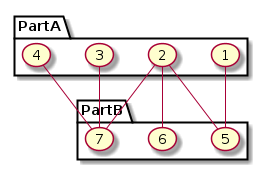
\includegraphics[scale=0.5]{ressources/images/BipartiteGraph.png}
            \caption{A bipartite graph (With its 2 parts)}
            \label{Bipartite graph}
        \end{figure}
    \subsection{Bipartite $\Leftrightarrow$ no odd cycle}
        \subsubsection{Definition}
            $G$ is bipartite $\Leftrightarrow G$ has no odd cycle
        \subsubsection{Proof}
            \begin{itemize}
                \item $\Rightarrow$: trivial
                \item $\Leftarrow$: Induction on $|E(G)|$\\
                    If $|E(G)|=0$, trivial\\
                    Let $e\in E(G)$\\
                    $G\backslash e$ has no odd cycle $\Rightarrow$ $G\ e$ is bipartite\\
                    $G\backslash e$ has a bipartition ($A, B$)\\
                    We may assume both ends are in $A$\\
                    If$G\backslash e$ has a path $P$ from $x$ to $y$, length of $P$ is even.\\
                    $P+e:=\text{odd cycle}$
            \end{itemize}

\chapter{Bipartite graph}
    \section{Complete bipartite graph}
        Let's call $K_{m,n}$a complete bipartite graph
        \begin{figure}[h]%TODO
            \centering
            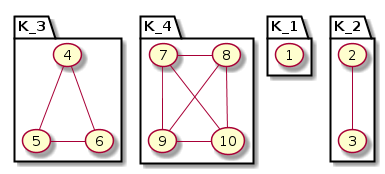
\includegraphics[scale=0.5]{ressources/images/CompleteGraphs.png}
            \caption{Every complete graph from $K_0$ to $K_4$}
            \label{Complete graph}
        \end{figure}
    \section{Euler tours}
        \subsection{Definition}
            A circuit is \textbf{Eulerian} if it contains every edge
        \subsection{Theorem}
            $G$ has a Eulerian circuit $\Leftrightarrow G\backslash$ (isolated vertices) is coonnected and every vertex has even degree
        \subsection{Proof}
            \begin{itemize}
                \item $\Rightarrow$: We may assume $G$ has no isolated vertices $\Rightarrow$ $C$ contains a walk from $v$ to $w$
                \item $\Leftarrow$: Induction on $|V(G)|+|E(G)|$\\
                    We may assume $G$ is connected (by removing isolated vertices)\\
                    We may assume $|V(G)|>1$\\
                    $G$ contains a cycle $C$ (Else, it would be a tree)\\
                    By the induction hyp, each non trivial component of $H$ has an Eulerian circuit
            \end{itemize}


\chapter{Matchings}
    A \textbf{matching} of a graph $G$ is a set of non-loop edges such that no 2 edges share an end.\\
    $\emptyset$ is a matching
    \section{Matching in a bipartite graph}
        \begin{description}
            \item[$\nu(G)$]: max size (number of edge) of a matching of $G$\\
                \begin{figure}[h]
                    \centering
                    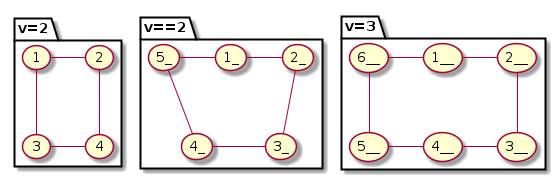
\includegraphics[scale=0.5]{ressources/images/NuG.png}
                    \caption{Examples of $\nu(G)$}
                    \label{Tree}
                \end{figure}
            \item[$\tau(G)$]: min number vertices that meet every edge\\
                ($min|x|:x\subseteq V(G)$ every edge has at least 1 end in $X$)
            \item[$M$-alternating path] is a path $P=v_0 e_1 v_1 e_2 v_2 e_3 v_3 e_4 \cdots e_n v_n$ such that $e_2, e_3, \cdots \in M$
            \item[$M$-augmenting path] is a path $P=v_0 e_1 v_1 e_2 v_2 e_3 v_3 e_4 \cdots e_n v_n$ such that $P$ is $M$-alternating and $V_0 V_n$ are not incident with any edge in $M$
        \end{description}
        \subsection{König's theorem}
            $G$ bipartite $\Rightarrow$ $\nu(G)=\tau(G)$
        \subsection{Proof}
        \subsection{Lemma}
            Let $M$ be a matching of a graph $G$\\
            $M$ is a maximum matching $\Leftrightarrow$ $G$ has no $M$-augmenting path
        \subsection{Proof}
            \begin{description}%TODO: finish
                \item[$\Rightarrow$] If $P$ is an $M$-augmenting path\\
                    Let $M'=M\Delta E(P)$ ($X\Delta Y=(X-Y)\cup(Y-X)$)\\
                \item[$\Leftarrow$]: \textbf{$\tau(G)\geq \nu(G)$}: Trivial (Even works for all graphs)\\
                \textbf{$\tau(G)\leq \nu(G)$}: Let $k=\nu(G)$\\
                        Let $M$ be a matching of size $k$.\\
                        \textbf{We want to find a set of $k$ vertices meeting every edges}
                        Let $(A, B)$ be a bipartition of $H$\\
                        \textit{$G$ has no $M$-augmenting path}

                        Let $A'=A-V(M)$\\
                        Let $B_0$ be the subset of $B$ that can be reached from $A'$ by an $M$-alternating path.\\
                        Let $A_0=$subset of $A$ incident with an edge in $M$\\
                        Let $A_1=A-A_0-A'$\\
                        \textbf{CLAIM}: Every edge is incident with a vertex in $A_1\cap B_0$ $\Rightarrow$ \textbf{TRUE}
            \end{description}
        \subsection{Hall's theorem}
            Let $G$ be a bipartite grpah with a bipartition $(A, B)$\\
            $G$ has a matching $M$ covering $A$ $\Leftrightarrow$ $\forall S \subseteq A, |N_{G}(S)|\geq|S|$ (With $N_{G}(S)$=set of all neighbours of $G$ vertices in $S$)\\
        \subsection{Proof}
            \begin{description}
                \item[$\Leftarrow$]: König's theorem show that $\nu(G)=|A| \Rightarrow \tau(G)=|A|$
                \item[$\Rightarrow$]:
            \end{description}
        \subsection{Other proof}
            Induction on $|A|$\\
            \begin{description}
                \item[Case 1]: $|N_{G}(S)|>|S|$\\
                    $\forall \phi \in S\subsetneq A$, let's choose $x\in A, y\in B$ such that $x$ and $y$ are adjacents\\
                    Let $H=G\backslash x\backslash y$\\
                    For $\phi\neq S\subseteq A-\{x\}$\\
                    $\begin{array}{r l}
                        |N_{H}(S)|&\geq|N_{G}(S)|-1\\
                        &\geq(|S|+1)-1=|S|
                    \end{array}$
                    By induction, $H$ has a matching M covering $A-\{x\}$\\
                    $M\cup\{xy\}$ is a matching of $G$ covering $A$
                \item[Case 2]: There is a set $A_0\subsetneq A$ such that $|N_{G}(A_0)|=|A_0|$\\
                    By induction, there is a matching $M_1$ covering $A_0$\\
                    Let $S\subseteq A-A_0$\\
                    Let $H=G\backslash A_0 \backslash N_{G}(A_0)$\\
                    \textbf{Goal}: $|N{H}(S)|\geq|S|$?\\
                    $\begin{array}{r c l}
                        |N_G(A_0\cup S)|&=&|N-G(A_0)|\\
                        &=&|A_0|+|N_H(S)|\\
                        &\geq&|A_0|+|S|
                    \end{array}$
            \end{description}
        \subsection{Def: $k$-regular}
            $G$ is \textbf{k-regular} if every vertex has degree $k$
        \subsection{Def: Perfect matching}
            A matching is \textbf{perfect} if it covers every vertex
        \subsection{Corrolary}
            Every $k$-regular bipartite graph has a parfect matching
        \subsection{Proof}
        \subsection{Petersen's corrolary}
            $k$: even, $\geq 2$\\
            \textbf{Every $k$-regular} graph has a spanning 2-regular subgraph.\\
        \subsection{Proof}
            $G$ has an Eulerian circuit $C$.\\
            We orient edges according to $C$.\\
            Construct a bipartite graph on $V\cup V'$ (Where $V'$ is a copy of $V$)
    \section{Matching in a general graph}
        \textbf{When do we have a perfect matching ?}\\
        \begin{itemize}
            \item $|V(G)|$ is even
            \item No isolated vertices
            \item No odd components
        \end{itemize}
        \subsection{Tutte theorem}
            $G$ has a perfect matching $\Leftrightarrow$ $odd(G\backslash S)\leq|S| \forall S\subseteq V(G)$\\
            (Where $odd(G)$ is the number of odd component of $G$)
        \subsection{Proof}
            \begin{description}
                \item[$\Rightarrow$]: trivial
                \item[$\Leftarrow$]: Induction on $|V(G)|$\\
                    \begin{enumerate}
                        \item $|V(G)|$is even\\
                            \textbf{Proof:} $odd(G)\leq 0$\\
                            Let's call $X$ critical if $odd(G\backslash X)=|X|$\\
                            $G$ has a critical set ($\emptyset$)
                        \item If $odd(G\backslash X)\geq |X|-1$, then $X$ is critical\\
                            \textbf{Proof:} $0\cong |V(G| \cong odd(G\backslash X)+|X|$ (mod 2)\\
                            Choose a maximal ciritcal set $X$\\
                            $C_1\cdots C_K$: odd components of $G\backslash X$\\
                            $D_1\cdots D_K$: even components of $G\backslash X$\\
                            $k=|X|$
                        \item $G\backslash X$ has no even component\\
                            \textbf{Proof:} Otherwise, let $v\in V(\text{even componenent }D)$\\
                            $odd(G\backslash (X\cup{v}))\geq|X|$
                        \item $\forall i \in 1, \cdots, k$, each $v\in V(C_i)$, $C_i\backslash v$ has a perfect matching.\\
                            \textbf{Proof:} If not, then there is a set $Y\subseteq V(e_i)-\{v\}$\\
                            $odd(V_i-{v}-Y)>|Y|$\\
                            Let $X'=X\cup Y\cup{v}$\\
                            $odd(G\backslash X')\geq(|X|-1)+(|Y|_1)$
                    \end{enumerate}%TODO: finish list(part 4)
            \end{description}
        \subsection{Cut edge}
            An edge e is a \textbf{cut-edge} if $G\backslash e$ has more components than $G$
        \subsection{Petersen's Corrolary (1891)}
            \textbf{Q:} Does every 3-regular graph have a perfect matching?\\
            \textbf{A:} False, we can found some counter-example\\
            But... If $G$ is a \textbf{simple} 3-regular graph, with at most 2 cut-edges, then $G$ has a perfect matching
        \subsection{Proof}
            Suppose $X\subseteq V(G)$.\\
            $odd(G\backslash X)>|X|$\\
            \begin{itemize}
                \item Each component of $G$ has even number of vertices.
                \item Let's take a look a one particular componenet.\\
                    If $C$ is an odd component of $G\backslash X$, then the number of edges from $X$ to $C$ is odd\\
                    $3|V(C)|=2|E(C)|+$(number of edges from $X$ to $C$)\\
                    Let's go back to every component.\\
                    $3(K-2)+2\leq\text{(Number of edges from X to odd components)}\leq 3|X|$\\
                    $\Leftrightarrow |X|\leq k\leq|X+1|$
                    $\Leftrightarrow k=|X+1|$\\
                    \textbf{But}, we also have:\\
                    $odd(G\backslash X)+|X|\cong |V(G)|$ (mod 2)\\
                    $\Leftrightarrow|V(G)|\cong 0$ (mod 2)\\
                    $\Leftrightarrow|V(G)|\cong |X|$ (mod 2)\\
                    \textbf{Contradiction}
            \end{itemize}
        \subsection{Tutte-Berge formula}
            $|V(G)|-2\nu(G)=\max_{X\in V(G)}(odd(G\backslash X)-|X|)$
        \subsection{Proof}
            \begin{itemize}
                \item $\geq$: trivial
                \item $\leq$: Let $k=\max(odd(G\backslash X)-|X|)$\\
                    Goal: find a matching of size $\frac{|V(G)|-k}{2}$\\
                    $G'$ is obtained from $G$ by adding a complete graph on k vertices and making new vertices adjacent to all new vertices.\\
                    Enough to show that $G'$ has a perfect matching.\\
                    $odd(G'\backslash X)\leq 1$\\
                    If $X$ does not contain all new vertices, then $odd(G')=0$\\
                    If $X$ contains all new vertices,\\
                    $\begin{array}{r c l}
                        odd(G'\backslash X) &=& odd(G\backslash (X\cap V(G)))\\
                        &\leq&|X\cap V(G)|+k\\
                        &\leq&|X|
                    \end{array}$
            \end{itemize}
        \subsection{Other proof}
            Let $f_G(U):=$number of vertices in odd components of $G\backslash U$\\
            Choose U such that:\\
            \begin{itemize}
                \item $|V(G)|+2\nu(G)=odd(G\backslash U)-|U|$\\
                \item Minimizing $f_G(U)$
            \end{itemize}
        \subsection{Properties}
            \begin{itemize}
                \item All even componenets of $G\backslash U$ have perfect matchings.\\
                \item \textbf{CLAIM}: If $C$ is a component of $G\backslash U$, and  $v\in V(C)$, then$C\backslash v$ has a perfect matching.\\
                    If not, then there is $X\subseteq V(C)-\{v\}$ such that $odd(C\backslash X \backslash V)>|X|$
                \item By the parity, $odd(C\backslash X \backslash V)\geq |X|+2$.\\
            \end{itemize}
        \subsection{Claim}
            Fr every non empty subset $W$ of $U$, number of odd componenet of $G\backslash U$ having neighbours in > $\geq |W|+1$
        \subsection{Gallait-Edmond Sctructure Theorem}
            Define $D, A, C$ as :\\
            \begin{itemize}
                \item D(G) = Vertices in odd component of $G\backslash U$
                \item A(G) = U
                \item C(G) = vertices in even components of $G\backslash U$
            \end{itemize}
            Then:\\
            \begin{enumerate}
                \item For each component $C$ of $G[D(G)]$ and each vertex $v$ of $C$, $C\backslash v$ has a perfect matching.\\
                \item $G[C(G)]$ has a perfect matching\\
                \item For all $\phi\neq S\leq A(G)$, $S$ has $\geq|S|+1$ components of $G[D(G)]$ having neighbours of $S$.
                \item $|V(G)|-2\nu(G)=odd(G\backslash A(G))-|A(G)|$
            \end{enumerate}
        \subsection{Lemma}
            Let $P$ be a path from $x$ to $y$ in $G$, where $y$ is adjacent to a vertex $z$ not covered by $M$\\
            Then one of the followings holds:\\
            \begin{enumerate}
                \item $G$ has a $M$-augmenting path from $x$ to $z$\\
                \item $G$ has a $M$-flower from $x$
            \end{enumerate}
            A $M$-flower is an $M$-alternating walk $P=v_0v_1\cdots v_n$ such that $v_0, \cdots, v_{n-i}$ are distinct, and $v_n=v_i$ for some $i<n$
        \subsection{Cycle shrinking Lemma}
            Let $G$ be a simple graph.\\
            $M$ be a matching.\\
            $C$ be a cycle with $2k+1$ edges such that exactly $k$ edges of $C$ are in $M$\\
            And 1 vertex is not covered by $M$\\
            Then: 
            \[
                M\text{ is a maximum matching of }G\Leftrightarrow M-E(C)\text{ is a maximum matching of }G\backslash E(C)
            \]
        \subsection{Stable matching}
            For each vertex $x$ of $G$, let us give a linear ordering $\leq_{v}$ of the edges incident with $v$ (i.e.: $e\leq_v f\Rightarrow v$ prefers $f$ to $e$)\\
            $M$ is \textbf{stable} if there is no edge $e\in E(G)\backslash M$ such that for each end $v$, there is $f\in M$ incident with $v$ and $f\leq_v e$
        \subsection{Gale-Shapley theorem}
            Every simple bipartite graph has a stable matching
        \subsection{$\Rightarrow$ Algorithm for Gale-Shapley theorem}
            \begin{description}
                \item[Step 2i] Every single boy proposes to the best girl tha he never proposed to
                \item[Step 2i+1] Each girl chooses the best boy among all boys who proposed to her at state $2i$, and the current partener
            \end{description}
            And we loop to step $2i+2$\\

\chapter{Connectivity}
    \section{Definition}
        \subsection{$k$-connected}
            A graph is \textbf{$k$-connected} if:\\
            \begin{enumerate}
                \item $|V(G)|>k$
                \item $G\backslash X$ is connected for all $X\subseteq V(G)$ with $|X|<k$
            \end{enumerate}
        \subsection{Cut edge}
            If $G\backslash v$ has more components than $G$, then $v$ is a \textbf{cut-vertex} if $G$
        \subsection{$k$-edge-connected}
            $\delta_G(X)$ = set of all edges having one end in $X$ and another end in $V(G)\backslash X$
            If $G$ is a \textbf{$k$-edge-connected} graph, then $|\delta_G(X)|\geq k \forall \emptyset \neq X \subsetneq V(G)$
        \subsection{$2$-edge-connected}
            \subsubsection{Lemma}
                Let $x, y\in E(G)$\\
                If $G$ has a cycle $D$ containing $y$ and $z$, then $G$ has a cycle containing $x$ and $z$
            \subsubsection{Theorem}
                Let $G$ be a connected graph with >2 vertices\\
                The following are equivalent :\\
                \begin{enumerate}
                    \item $G$ is 2-connected
                    \item If $e, f$ are non-loop edges, then $G$ has a cycle containing $e$ ad $f$
                    \item If $v, w$ are vertices of $G$, then $G$ has a cycle containing $v$ and $w$
                \end{enumerate}
            \subsubsection{Property}
                Let $e$ be an edge of a 2-connected graph $G$\\
                Then, either $G\backslash e$pr $G/e$ is 2-connected, unless $|V(G)|=3$
            \subsubsection{Theorem}%TODO :perhaps some thm left
            \subsubsection{Menger's theorem}
                $G$ gas at least $k$ disjoint paths from $S$ to $T$\\
                $\Leftrightarrow$\\
                $G$ has no $x\subseteq V(G)$ such that $|x|<k$ and $G\backslash x$ has no path from $s-x$ to $t-x$
            \subsubsection{Menger's theorem corrolary}
                Let $a, b$ be non-adjacent pair of dinstinct vertices of $G$.\\
                $G$ has $k$ iternally distinct path from $a$ to $b$\\
                $\Leftrightarrow$\\
                $G$ has no set $S$, $|S|<k, S\subseteq V(G)-\{a, b\}$, such that $G\backslash S$ has no path from $a$ to $b$
            \subsubsection{Corrolary}
                Let $G$ be a graph with >$k$ vertices :\\
                $G$ is $k$-connected\\
                $\Leftrightarrow$\\
                $\forall\text{ pairs }a,b$ of distinct vertices, $G$ has $k$ internally paths from $a$ to $b$
        \subsection{$3$-connected}
            \subsubsection{Theorem}
                If $G$ is $3$-connected and $|V(G)|>4$ , then $G$ has an edge $e$ such that $G/e$ is $3$-connected
            \subsubsection{Tutte's chain theorem}
                Let $G$ be a simple $3$-connected graph.\\
                Then, there exists an edge $e$ such that either $G\backslash e$ or $G/e$ is simple $3$-connected (unless $G$ is the ``Wheel'')\\
                (The ``Wheel'' is a cycle + a vertex adjacent to every other vertex)
                \subsubsection{Seymour's splitter theorem}

\chapter{Plane graphs}
    \section{General definition}
        \begin{description}
            \item[Plane graph] A plane graph is a graph $(V, E)$ such that:
                \begin{itemize}
                    \item $V\subseteq \mathbb{R}^2$ (vertices are part of the plane)
                    \item Every edge is an arc joining 2 vertices
                    \item The interior of each edge contains no vertex and no interior point of other edges
                \end{itemize}
            \item[Planar graph] A graph is planar if it is isomorphic to a plane graph.
            \item[Drawing] If $G$ is a surface, a drawing of a graph $G$ on $S$ is a mapping from $G$ so that vertices are mapped to distinct point of $S$, and each edge is mapped to an arc joining 2 points corresponding to the ends.\\
            \item[Map] A drawing without any edge crossing is called a map (or an embedding).\\
            \item[Embeddable] $G$ is ``embeddable'' on $S$ if there is \\
        \end{description}
    \section{Lemma}
        If $G$ is a 2-connected loopless plane graph, then every face boundary is a cycle of $G$, and each edge is incident with exactly 2 faces.
    \section{Euleur formula}
        \subsection{Euleur formula}
            If $G$ is a connected plane graph with :
            \begin{itemize}
                \item $v$ vertices
                \item $e$ edges
                \item $f$ faces
            \end{itemize}
            then $v-e+f=2$
        \subsection{$\searrow$Corrolary}
            If $G$ is a simple plane graph, then:\\
            $|E(G)|\leq 3|V(G)|-6$, unless $|V(G)|\leq 2$
        \subsection{$\searrow$Use example}
            \begin{itemize}
                \item $K_5$: $3-5-6< 10$ $\Rightarrow$ $K_5$ is nonplanar
            \end{itemize}
        \subsection{$\searrow$Corrolary}
            If $G$ is a simple plane graph with no triangle (cycle of length 3), then:\\
                $|E(G)|\leq 2|V(G)|-4$, unless $|V(G)|\leq 2$
    \section{Kuratowski theorem and $K_5$/$K_{3, 3}$ ``things''}
        \subsection{Kuratowski theorem}
            A graph is planar $\Leftrightarrow$ it has a $K_5$ or $K_{3, 3}$ topological minor.
        \subsection{$\searrow$Wagner-Kuratowski corrolary}
            A graph is planar $\Leftrightarrow$ it has a $K_5$ or $K_{3, 3}$ minor.
        \subsection{Convex embedding}
            \begin{itemize}
                \item Evey edge is mapped to a straight-line segment
                \item Every inner face is convex
                \item Then complement of the outer face is convex
            \end{itemize}
        \subsection{$\searrow$Property}
            If $G$ is a simple 3-connected graph with no topological minor isomorphic to $K_5$ or $K_{3, 3}$, then\\
            $G$ has a convex embedding on $\mathbb{R}^2$
        \subsection{Lemma}
            If $G/e$ has a $K_5$ topoligical minor, then $G$ has a $K_5$ OR $K_{3, 3}$ topoligical minor
        \subsection{Lemma}
        If $G/e$ has a $K_{3, 3}$ topoligical minor, then $G$ has a $K_{3, 3}$ topoligical minor
    \section{Dual graph}
        \subsection{Dual graph}
            For a given plane graph $G=(V, E)$, the geometric dual $G^*$ of $G$ is a graph $H$ such that:
            \begin{enumerate}
                \item every face of $G$ has precisely 1 vertex of $H$
                \item For every edge $e$ of $G$, $H$ has a unique edge $e^*$ that crosses $e$ and joins 2 vertices of $H$ that are in the faces incident with $e$, and no other edges of $H$ meet $e$
                \item $*:E(G)\rightarrow E(G^*)$ is a bijection
            \end{enumerate}
        \subsection{$\searrow$Lemma}
            If $G$ is a plane graph, then $G^*$ is connected.
        \subsection{$\searrow$Theorem}
            Let $G$ be a connected plane graph.\\
            If $H$ is the geometric dual of $G$, then $G$ is the geometric dual of $H$
        \subsection{Abstract dual}
            $H$ is called an abstract dual of $G$ if it exists a bijection
            \[*:E(G)\rightarrow E(H)\]
            such that 
            \[F\subseteq E(G)\text{ is the edge set of a cycle of }G\Leftrightarrow F^*\text{ is a minimal nonempty adjacent of }H\]
        \subsection{$\searrow$Property}
            If $H$ is the geometric dual of $G$, then $H$ is an abstract dual of $G$
        \subsection{$\searrow$Theorem}
            If $H$ is the abstract dual of $G$, then $H$ is an abstract dual of $G$
        \subsection{Whitney theorem}
            $G$ has an abstract dual $\Leftrightarrow$ $G$ is planar

\chapter{Graph coloring}
    \section{Vertex coloring}
        \subsection{Definition}
            \begin{description}
                \item[k-coloring]: A $k$-coloring of a graph $G$ is a fonction $c:\nu(G)\rightarrow\{1, 2, \ldots, k\}$ such that $\forall$ edge $e=uv$, $c(u)\neq c(v)$
                \item[k-colorable]: A graph $G$ is k-colorable if it has a $k$-coloring.
                \item[$\chi$(G)]: The chromatic number $\chi(G)$ of a graph $G$ is the minimum $k$ such that $G$ has a $k$-coloring.
                \item[Stable set]: A set $X\subseteq V(G)$ is called stable if no 2 vertices in $X$ are adjacent
                \item[Maximum degree] Let's call $\Delta(G)=\max_{v\in V(G)}{deg_G(v)}$
            \end{description}
        \subsection{Loopfull G}
            If $G$ contains a loop, then $G$ is NOT colorable, and $\chi(G)=\infty$
        \subsection{Loopless G}
            If $G$ is loopless, then 
                \[\chi(G)\leq \Delta(G)+1\]
        \subsection{Theorem: Colorability of planar graph}
            Every simple planar graph is 5-colorable.
        \subsection{Theorem: Brook}
            If $G$ is simple, connected, then
                \[\chi(G)\leq\Delta(G)\]
            Unless $G$ is the complete graph or the odd cycle.
    \section{Edge coloring}
        \subsection{Definition}
            \begin{description}
                \item[k-edge-coloring] of a graph G is a function $c:E(G)\rightarrow \{1, 2, \cdots, k\}$ such that $c(e)\neq c(f)$ whenever e and f share a vertex.
                \item[k-edge-colorable] is a graph G if it has a k-edge-coloring
                \item[$\chi$'] is the edge chromatic number/index=min k such that G has a k-edge-coloring
            \end{description}
        \subsection{König's theorem}
            If $G$ is biparite, $\chi'(G)=\Delta(G)$
        \subsection{Vizing theorem}
            If $G$ is simple, then $\chi'(G)=\Delta(G)\text{ or }\Delta(G)+1$
        \subsection{$\searrow$Lemma}
            Let $G$ be a simple graph with $\Delta(G)\leq k$\\
            Let $v$ be a vertex of $G$\\
            Let $e_1, e_2, \cdots, e_n$ be some edges incident with $v$\\
            Then $G$ is k-edge-colorable
        \subsection{$\searrow$Prop}
            Lemma$\Rightarrow$Theorem: Take $k=\Delta(G)+1$
    \section{List coloring}
        \subsection{Definition}
            \begin{description}
                \item[List assignement] of a graph $G$ is a function that match each vertex $v$ to a list $L(v)$ of color
                \item[L-list coloring] of $G$ is a function on $V(G)$ such that$c(v)\in L(v)$ and $c(u)\neq c(v)$ whenever $u$ and $v$ are adjacent
                \item[k-list colorable] is a graph $G$ if for all list assigments $L$, with $|L(v)[\geq k \forall \text{ vertex }v$, $G$ has a L-list coloring
                \item[$\chi_l(G)$] = min k such that $G$ is k-list-colorable
            \end{description}
        \subsection{Theorem}
                $k-list-colorable \Rightarrow k-colorable$\\
                $k-list-colorable \not\Leftarrow k-colorable$\\
                $\chi(G)\leq\chi_l(G)$
        \subsection{Theorem}
            Every simple planar graph is $5-list-colorable$
        \subsection{Alan T~ Theorem}
            Every bipartite planar graph is $3-list-colorable$
        \subsection{List coloring conjecture}
            ``List edge-chromatic index'' $\Leftrightarrow$ $\chi_l'(G)$ or ch'$(G)$
        \subsection{Galvin's theorem}
            Let $G$ be a simple bipartite graph. Then:
            \[
                \Rightarrow \chi-l'(G)=\chi'(G)
            \]
    \section{Perfect graphs}
        \subsection{Definitions}
            \begin{description}
                \item[Clique] is a set of vertices pairwise adjacent
                \item[$\omega(G)$] is the maximum size of a clique in $G$. We know that $\chi(G)\geq\omega(G)$
            \end{description}
        \subsection{Theorem Erdois}
            For $k, l$, there is a graph $G$ such that $\chi(G)>k$ and $G$ has no cycle of length $\leq l$
        \subsection{Simple graph}
            A simple graph $G$ is perfect if:\\
            \[
                \chi(H)=\omega(H)
            \]
            For every induced subgraph $H$ of $G$
        \subsection{Examples of perfect graph}
            \begin{enumerate}
                \item Bipartite graph
                \item Complement of a bipartite graph\\
                \item Line graph of a bipartite graph $L(G)$\\
                    \[
                   \left.
                       \begin{array}{lcr}
                            \chi(L(G))=\chi(G)&=& \Delta(G)(Konig)\\
                            \omega(L(G)) &\geq& \Delta(G)
                        \end{array}
                    \right\} \Rightarrow \chi(L(G))\leq\omega(L(G))
                \]
                \item Complement of a line graph of a bipartite graph
                    \[
                   \left.
                       \begin{array}{lcr}
                           \chi(\overline{L(G)}) &\leq& \tau(G)\\
                           \omega(\overline{L(G)}) &=& \nu(G)
                        \end{array}
                    \right\} \Rightarrow \chi(\overline{L(G)})\leq\omega(\overline{L(G)})
                \]
            \end{enumerate}
        \subsection{Strong Perfect Graph Conjecture}
            $G$ is perfect $\Leftrightarrow$ $G$ has no ``odd hole'' and no ``odd antihole''
        \subsection{Lovàisz theorem 1}
            If $G$ is perfect, then $\overline{G}$ is perfect.
        \subsection{$\searrow$Lemma}
            If $G$ is minimally imperfect, then for every stable set $U$ of $G$:
            \[
                \omega(G\backslash U)=\omega(G)
            \]
        \subsection{Lovàisz theorem 2}
            $G$ is perfect $\Leftrightarrow$ $\alpha(H)\omega(H)\geq|V(G)|$

\chapter{Nowhere-zero Flows}
    \section{Definition}
        \begin{description}
            \item[Circulation] Let $D$ be a directed graph.\\
                A circulation $\phi$ of $D$ is a function $\phi:E(D)\rightarrow \mathbb{R}$, such that for each vertex $v$ of $D$:
                \[
                    \sum_{e\in\delta^+(v)}\phi(e)=\sum_{e\in\delta^-(v)}\phi(e)
                \]
            \item[Nowhere zero $k$-flow] For a positive integer $k$, a nowhere zero $k$-flow of $D$ is a circulation $\phi$ such that:
                \[
                    |\phi(e)|\in \{1, 2, \ldots, k-1\}
                \]
            \item[Nowhere $\mathbb{Z}_k$-circulation] A $\mathbb{Z}_k$-circulation is a function $\phi:E(G)\rightarrow \mathbb{Z}_k$ such that:\\
                \[
                    \sum_{e\in\delta^+(e)}=\sum_{e\in\delta^-(e)}\text{ (mod k)}
                \]
            \item[Nowhere zero $\mathbb{Z}_k$-flow] A $\mathbb{Z}_k$-flow is a $\mathbb{Z}_k$-circulation such that $\phi(e)\neq0$ (mod k) for all edge $e$
            \item[Nowhere $\Gamma$-circulation] A $\mathbb{Z}_k$-circulation is a function $\phi:E(G)\rightarrow \Gamma$ such that:\\
                \[
                    \sum_{e\in\delta^+(e)}=\sum_{e\in\delta^-(e)}\text{ (mod k)}
                \]
            \item[Nowhere zero $\Gamma$-flow] A $\Gamma$-flow is a $\Gamma$-circulation such that $\phi(e)\neq0$ (mod k) for all edge $e$
        \end{description}
        (nb: $\mathbb{Z}_k = \{0, 1, \cdots, k-1\}$)
    \section{Theorem}
        Let $G$ be a plane graph. Then $G^*$(Geometric dual) is $k$-colorable $\Leftrightarrow$ $G$ has a nowhere zero $k$-flow\\
    \section{Theorem}
        $G$ has a nowhere zero $k$-flow $\Leftrightarrow$ $G$ ahs a nowhere zero $\mathbb{Z}_k$-flow
    \section{$\searrow$Corrolarry 1}
                if $k'>k$, and $g$ has a nowhere zero $k$-flow $\rightarrow$ $g$ has a nowhere zero $k'$-flow
    \section{$\searrow$Corrolarry 2 ($\mathbb{Z}_k$)}
        if $k'>k$, and $g$ has a nowhere zero $\mathbb{Z}_k$-flow $\rightarrow$ $g$ has a nowhere zero $\mathbb{Z}_{k'}$-flow
    \section{$\searrow$Corrolarry 3 ($\Gamma$)}
        $G$ has a nowhere zero $\Gamma$-flow $\Leftrightarrow$ $G$ has a 
    \section{$\searrow$Corrolarry 4 ($\Gamma$)}
        $|\Gamma_1|<|\Gamma_2|$. $G$ has a nowhere zero $\Gamma_1$-flow $\Rightarrow$ $G$ has a nowhere zero $\Gamma_2$-flow


\pageQuatriemeCouverture{}
\end{document}
